\section{Результат работы алгоритма}

\begin{figure}
  \centering
  \subbottom[bunny with noise]{%
    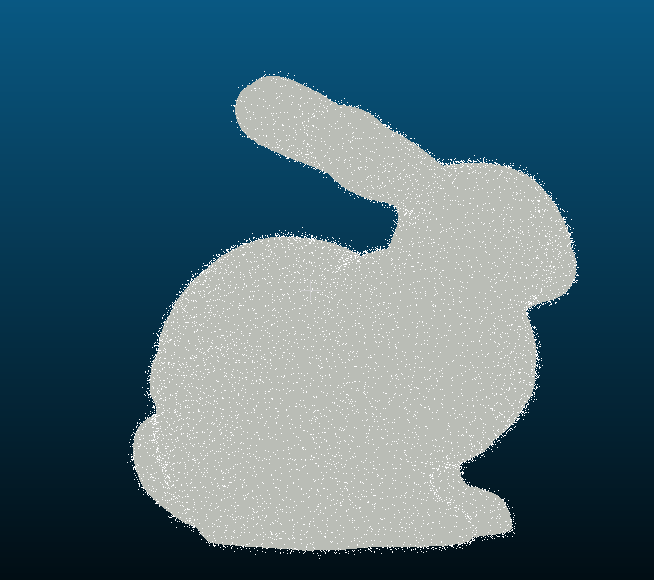
\includegraphics[width=8cm]{images/bunnyWithNoise.png}}
  \subbottom[bunny after MLS]{%
    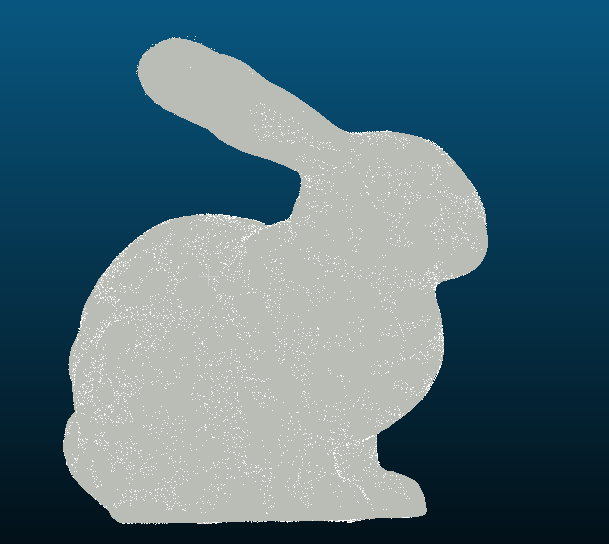
\includegraphics[width=8cm]{images/bynnyAfterMLS.png}}
  \caption{Слева зашумленное облако точек аддитивным Гауссовым шумом с $\boldsymbol{\sigma = 0.9}$ на эталонной поверхности. Справа, восстановленное облако точек методом MLS на той же эталонной поверхности.}
\end{figure}

\begin{figure}
  \centering
  \subbottom[bunny with noise]{%
    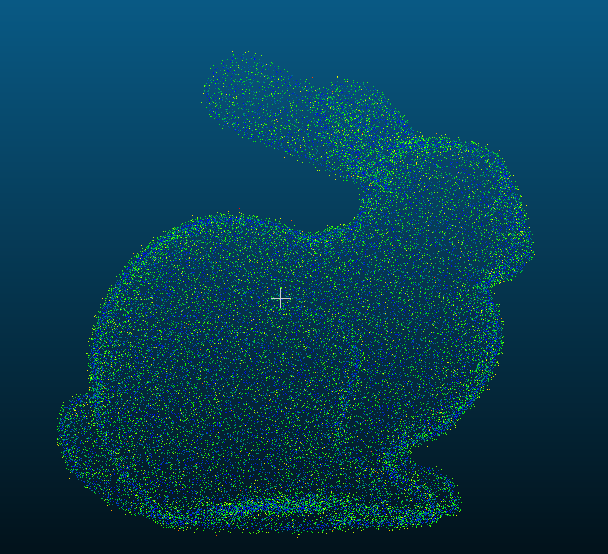
\includegraphics[width=8cm]{images/bunnyWithNoiseCompare.png}}
  \subbottom[bunny after MLS]{%
    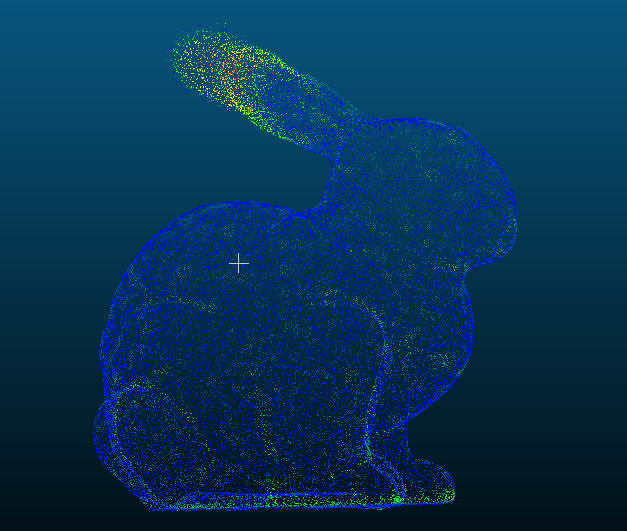
\includegraphics[width=8cm]{images/bunnyAfterMLSCompare.png}}
  \caption{Слева зашумленное облако точек аддитивным Гауссовым шумом с $\boldsymbol{\sigma = 0.9}$. Справа, восстановленное облако точек методом MLS. Интенсивность цвета обозначает величину отклонения от эталонной поверхности.}
\end{figure}

Для оценки работы алгоритма реконструкции поверхности, использовалась метрика геометрического отклонения. Были посчитаны среднеквадратичное отклонение точек от поверхности а также среднее расстояние.

\begin{center}
    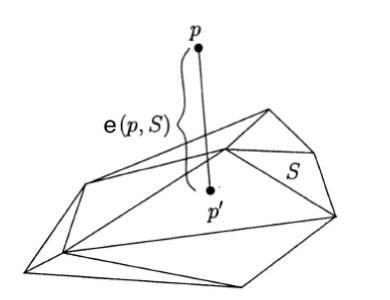
\includegraphics[width=0.8\textwidth]{images/distance.jpg}\\
    Метрика отклонения. Отклонение $e_i(p, S)$ — это расстояние атрибутов $i$ между точкой и поверхностью S. Точка $p^{'}$ — ближайшая точка к поверхности S.
\end{center}

\begin{table}[h!]
\centering
\begin{tabular}{|p{3cm} |p{2cm}| p{3cm} | p{2cm} | p{3cm}|}
    \hline
    metric & bunny with noise & bunny after MLS & brain with noise & brain after MLS \\
    \hline\hline
    std deviation & 0.901 & 0.383211 & 0.049 & 0.032\\
    \hline
    Mean distance & 0.721 &  0.286339 & 0.093 & 0.067\\
    \hline
\end{tabular}
\caption{Сравнение зашумленного и восстановленного методом MLS облака точек с эталонной поверхностью по std deviation и Mean distance.}
\label{table:1}
\end{table}

\begin{table}[h!]
\centering
\begin{tabular}{|p{3cm} |p{2cm}| p{3cm} |}
    \hline
    metric & trim-star with noise & trim-star after MLS \\
    \hline\hline
    std deviation & 0.475 &  0.329 \\
    \hline
    Mean distance & 0.382 &   0.267 \\
    \hline
\end{tabular}
\caption{Сравнение зашумленного и восстановленного методом MLS облака точек с эталонной поверхностью по std deviation и Mean distance. sd = 0.5 radius = 0.4}
\label{table:1}
\end{table}

\begin{table}[h!]
\centering
\begin{tabular}{|p{3cm} |p{2cm}| p{3cm} |}
    \hline
    metric & trim-star with noise & trim-star after MLS \\
    \hline\hline
    std deviation & 0.475 &  0.420 \\
    \hline
    Mean distance & 0.382 &   0.328 \\
    \hline
\end{tabular}
\caption{Сравнение зашумленного и восстановленного методом MLS облака точек с эталонной поверхностью по std deviation и Mean distance. sd = 0.5 radius = 1}
\label{table:1}
\end{table}

\begin{table}[h!]
\centering
\begin{tabular}{|p{3cm} |p{2cm}| p{3cm} |}
    \hline
    metric & trim-star with noise & trim-star after MLS \\
    \hline\hline
    std deviation & 0.291 &  0.205 \\
    \hline
    Mean distance & 0.233 &   0.165 \\
    \hline
\end{tabular}
\caption{Сравнение зашумленного и восстановленного методом MLS облака точек с эталонной поверхностью по std deviation и Mean distance. sd = 0.3 radius = 0.4}
\label{table:1}
\end{table}

\begin{table}[h!]
\centering
\begin{tabular}{|p{3cm} |p{2cm}| p{3cm} |}
    \hline
    metric & trim-star with noise & trim-star after MLS \\
    \hline\hline
    std deviation & 0.291 &  0.217 \\
    \hline
    Mean distance & 0.233 &   0.158 \\
    \hline
\end{tabular}
\caption{Сравнение зашумленного и восстановленного методом MLS облака точек с эталонной поверхностью по std deviation и Mean distance. sd = 0.3 radius = 1}
\label{table:1}
\end{table}

\begin{table}[h!]
\centering
\begin{tabular}{|p{3cm} |p{2cm}| p{3cm} |}
    \hline
    metric & trim-star with noise & trim-star after MLS \\
    \hline\hline
    std deviation & 0.100 &  0.086 \\
    \hline
    Mean distance & 0.08 &   0.068 \\
    \hline
\end{tabular}
\caption{Сравнение зашумленного и восстановленного методом MLS облака точек с эталонной поверхностью по std deviation и Mean distance. sd = 0.1 radius = 0.4}
\label{table:1}
\end{table}

\begin{table}[h!]
\centering
\begin{tabular}{|p{3cm} |p{2cm}| p{3cm} |}
    \hline
    metric & trim-star with noise & trim-star after MLS \\
    \hline\hline
    std deviation & 0.100 &  0.059 \\
    \hline
    Mean distance & 0.080 &   0.046 \\
    \hline
\end{tabular}
\caption{Сравнение зашумленного и восстановленного методом MLS облака точек с эталонной поверхностью по std deviation и Mean distance. sd = 0.1 radius = 1}
\label{table:1}
\end{table}


\begin{table}[h!]
\centering
\begin{tabular}{|p{3cm} |p{2cm}| p{3cm} |}
    \hline
    metric & Laurana with noise & Laurana after MLS \\
    \hline\hline
    std deviation & 5.458 &  4.707 \\
    \hline
    Mean distance & 4.001 &   3.192 \\
    \hline
\end{tabular}
\caption{Сравнение зашумленного и восстановленного методом MLS облака точек с эталонной поверхностью по std deviation и Mean distance. std = 5 radius = 10}
\label{table:1}
\end{table}

\begin{table}[h!]
\centering
\begin{tabular}{|p{3cm} |p{2cm}| p{3cm} |}
    \hline
    metric & Laurana with noise & Laurana after MLS \\
    \hline\hline
    std deviation & 5.458 &  4.383 \\
    \hline
    Mean distance & 4.001 &   2.810 \\
    \hline
\end{tabular}
\caption{Сравнение зашумленного и восстановленного методом MLS облака точек с эталонной поверхностью по std deviation и Mean distance. std = 5 radius = 4}
\label{table:1}
\end{table}

\begin{table}[h!]
\centering
\begin{tabular}{|p{3cm} |p{2cm}| p{3cm} |}
    \hline
    metric & Laurana with noise & Laurana after MLS \\
    \hline\hline
    std deviation & 3.806 &  3.036 \\
    \hline
    Mean distance & 2.445 &   1.422 \\
    \hline
\end{tabular}
\caption{Сравнение зашумленного и восстановленного методом MLS облака точек с эталонной поверхностью по std deviation и Mean distance. std = 3 radius = 10}
\label{table:1}
\end{table}

\begin{table}[h!]
\centering
\begin{tabular}{|p{3cm} |p{2cm}| p{3cm} |}
    \hline
    metric & Laurana with noise & Laurana after MLS \\
    \hline\hline
    std deviation & 3.806 &  3.635 \\
    \hline
    Mean distance & 2.445 &   1.880 \\
    \hline
\end{tabular}
\caption{Сравнение зашумленного и восстановленного методом MLS облака точек с эталонной поверхностью по std deviation и Mean distance. std = 3 radius = 4}
\label{table:1}
\end{table}

\begin{table}[h!]
\centering
\begin{tabular}{|p{3cm} |p{2cm}| p{3cm} |}
    \hline
    metric & Laurana with noise & Laurana after MLS \\
    \hline\hline
    std deviation & 2.60 &  2.451 \\
    \hline
    Mean distance &  0.900 &   2.397 \\
    \hline
\end{tabular}
\caption{Сравнение зашумленного и восстановленного методом MLS облака точек с эталонной поверхностью по std deviation и Mean distance. std = 1 radius = 10}
\label{table:1}
\end{table}

\begin{table}[h!]
\centering
\begin{tabular}{|p{3cm} |p{2cm}| p{3cm} |}
    \hline
    metric & Laurana with noise & Laurana after MLS \\
    \hline\hline
    std deviation & 2.60 &  2.592 \\
    \hline
    Mean distance &  0.900 &   0.810 \\
    \hline
\end{tabular}
\caption{Сравнение зашумленного и восстановленного методом MLS облака точек с эталонной поверхностью по std deviation и Mean distance. std = 1 radius = 4}
\label{table:1}
\end{table}